\documentclass[12pt]{amsart}
\usepackage{amsmath,amssymb,amsthm,hyperref,graphicx}
\usepackage[margin=1in]{geometry}
\usepackage{microtype}
\graphicspath{{figures/}}
\subjclass[2020]{Primary 57K32; Secondary 11R32, 11R04}
\keywords{hyperbolic 3-manifolds, invariant trace fields, Galois group,
  compositum, linear disjointness, Weyl groups}
\newtheorem{theorem}{Theorem}[section]
\newtheorem{lemma}[theorem]{Lemma}
\newtheorem{proposition}[theorem]{Proposition}
\newtheorem{corollary}[theorem]{Corollary}
\newtheorem{remark}[theorem]{Remark}
\DeclareMathOperator{\Gal}{Gal}
\DeclareMathOperator{\disc}{disc}
\newcommand{\Q}{\mathbb{Q}}
\newcommand{\Z}{\mathbb{Z}}
\newcommand{\C}{\mathbb{C}}
\title[Galois Product Structure of Trace Fields]{Arithmetic
  Disjointness and Galois Product Structure in a
  Family of Hyperbolic 3-Manifold Trace Fields}
\author{Marvin Gentry}
\address{Independent Researcher, Seattle, WA}
\email{drmlgentry@protonmail.com}
\urladdr{https://hyperbolicflavorgeometry.org}
\begin{document}
\begin{abstract}
We study the compositum of four number fields arising as invariant trace
fields of finite-volume cusped hyperbolic 3-manifolds selected by arithmetic
criteria.
The four fields have discriminants $-3$, $-283$, $-7$, and $-59$, with
individual Galois groups $C_2$, $S_4$, $C_2$, and $S_3$. We prove that
their Galois closures are jointly linearly disjoint over $\Q$ by two
independent methods: sequential degree multiplication verifying the chain
$144\to 288\to 576$, and a ramification argument using the pairwise
disjoint prime supports $\{3\}$, $\{283\}$, $\{7\}$, $\{59\}$ of the four
Galois pieces together with Minkowski's theorem. The Galois closure of the
compositum has degree $576$ with Galois group
$C_2\times S_4\times C_2\times S_3$. Via the standard Weyl group
identifications, this group is abstractly isomorphic to
$W(\mathrm{SU}(2))\times W(\mathrm{SU}(4))\times W(\mathrm{SU}(2))\times
W(\mathrm{SU}(3))$. All computations are verified in SageMath; reproducible
scripts are available at
\url{https://github.com/drmlgentry/hyperbolic-flavor-geometry}.
\end{abstract}
\maketitle

\section{Introduction}

The invariant trace field of a finite-volume hyperbolic 3-manifold is a
number-field invariant whose arithmetic encodes geometric data of the
manifold in a canonical way~\cite{MR}. For arithmetic hyperbolic
3-manifolds---those whose holonomy groups are arithmetic Kleinian
groups---the trace field and its Galois group carry particularly rigid
structure~\cite{NR}.

This paper concerns four hyperbolic 3-manifolds drawn from the SnapPy
census~\cite{SnapPy}, selected by arithmetic criteria arising in the
Hyperbolic Flavor Geometry research program~\cite{HFG}. Their invariant
trace fields are:
\begin{align*}
K_1 &= \Q(\sqrt{-3}), & \disc(K_1)&=-3,\\
K_2 &= \Q(\alpha),\quad\alpha^4-\alpha-1=0, & \disc(K_2)&=-283,\\
K_3 &= \Q(\sqrt{-7}), & \disc(K_3)&=-7,\\
K_4 &= \Q(\beta),\quad 8\beta^3-24\beta^2+28\beta-11=0, & \disc(K_4)&=-59.
\end{align*}
The individual Galois groups over $\Q$ are $C_2$, $S_4$, $C_2$, and $S_3$.

\begin{theorem}[Four-Field Galois Product Theorem]\label{thm:main}
Let $L_2$ denote the Galois closure of $K_2$ over $\Q$, and $L_4$ the
Galois closure of $K_4$ over $\Q$. Set $L = K_1 L_2 K_3 L_4$. Then
$L/\Q$ is Galois with
\[
\Gal(L/\Q)\cong C_2\times S_4\times C_2\times S_3,\qquad|\Gal(L/\Q)|=576.
\]
\end{theorem}

We give two independent proofs: a degree-multiplication argument
(Section~\ref{sec:degree}) and a ramification argument
(Section~\ref{sec:ramification}).

\begin{corollary}[Weyl Group Identification]\label{cor:weyl}
Using $W(\mathrm{SU}(2))\cong C_2$, $W(\mathrm{SU}(3))\cong S_3$,
$W(\mathrm{SU}(4))\cong S_4$,
\[
\Gal(L/\Q)\cong W(\mathrm{SU}(2))\times W(\mathrm{SU}(4))\times
W(\mathrm{SU}(2))\times W(\mathrm{SU}(3)).
\]
The identification of these factors with physical gauge sectors is discussed
in Section~\ref{sec:discussion} and is not part of the theorem.
\end{corollary}

\section{Preliminaries}\label{sec:prelim}

\subsection{Invariant trace fields}
For a hyperbolic 3-manifold $M$ with holonomy
$\rho\colon\pi_1(M)\to\mathrm{PSL}(2,\C)$, the invariant trace field
$k(M)$ is the subfield of $\C$ generated over $\Q$ by
$\{\mathrm{tr}(\rho(\gamma))^2:\gamma\in\pi_1(M)\}$.
It is an invariant of the commensurability class of $M$;
see~\cite[Chapter~3]{MR}.

\subsection{Linear disjointness and Galois products}
Extensions $E$, $F$ of $\Q$ are \emph{linearly disjoint} over $\Q$ if
$[EF:\Q]=[E:\Q][F:\Q]$.

\begin{lemma}\label{lem:product}
Let $E_1,\ldots,E_n$ be finite Galois extensions of $\Q$ that are jointly
linearly disjoint. Then $E_1\cdots E_n/\Q$ is Galois and
\[
\Gal(E_1\cdots E_n/\Q)\cong\prod_{i=1}^n\Gal(E_i/\Q).
\]
\end{lemma}
\begin{proof}
Standard; see e.g.~\cite[Theorem~1.14]{Neukirch}.
\end{proof}

\subsection{Ramification and Minkowski's theorem}
A rational prime $p$ ramifies in $K/\Q$ if and only if $p\mid\disc(K)$.
Minkowski's theorem asserts that every nontrivial finite extension of $\Q$
is ramified at at least one prime~\cite[Theorem~2.17]{Neukirch}.
Consequently, if two Galois extensions of $\Q$ have disjoint ramification
sets, their intersection is $\Q$.

\section{The Four Fields}\label{sec:fields}

\textbf{$K_1=\Q(\sqrt{-3})$.} The quadratic subfield of $\Q(\zeta_3)$.
Discriminant $-3$, $\Gal(K_1/\Q)\cong C_2$.

\textbf{$K_2=\Q(\alpha)$, $\alpha^4-\alpha-1=0$.} The polynomial
$x^4-x-1$ is irreducible over $\Q$ with discriminant $-283$. Its Galois
closure $L_2$ satisfies $[L_2:\Q]=24$ and $\Gal(L_2/\Q)\cong S_4$.

\textbf{$K_3=\Q(\sqrt{-7})$.} Discriminant $-7$, $\Gal(K_3/\Q)\cong C_2$.

\textbf{$K_4=\Q(\beta)$, $8\beta^3-24\beta^2+28\beta-11=0$.} An
irreducible cubic with number-field discriminant $-59$ (the polynomial
discriminant is $-3776=-64\cdot 59$; SageMath confirms the number-field
value). Its Galois closure $L_4$ satisfies $[L_4:\Q]=6$ and
$\Gal(L_4/\Q)\cong S_3$.

\begin{proposition}[Manifold--field identification]\label{prop:manifolds}
Using SnapPy's exact algebraic field-recognition routine, the invariant
trace fields of the cusped census manifolds $m003$, $m019$, $m010$, $m006$
are respectively $K_1$, $K_2$, $K_3$, $K_4$:
\[
k(m003)\cong K_1,\qquad k(m019)\cong K_2,\qquad k(m010)\cong K_3,\qquad
k(m006)\cong K_4.
\]
(For $m006$ the recognized defining polynomial is $x^3+2x-1$, which
SageMath confirms is isomorphic to $K_4$, with matching discriminant
$-59$.)
\end{proposition}

The four ramification sets $\{3\}$, $\{283\}$, $\{7\}$, $\{59\}$
are pairwise disjoint.
\begin{figure}[ht]
\centering
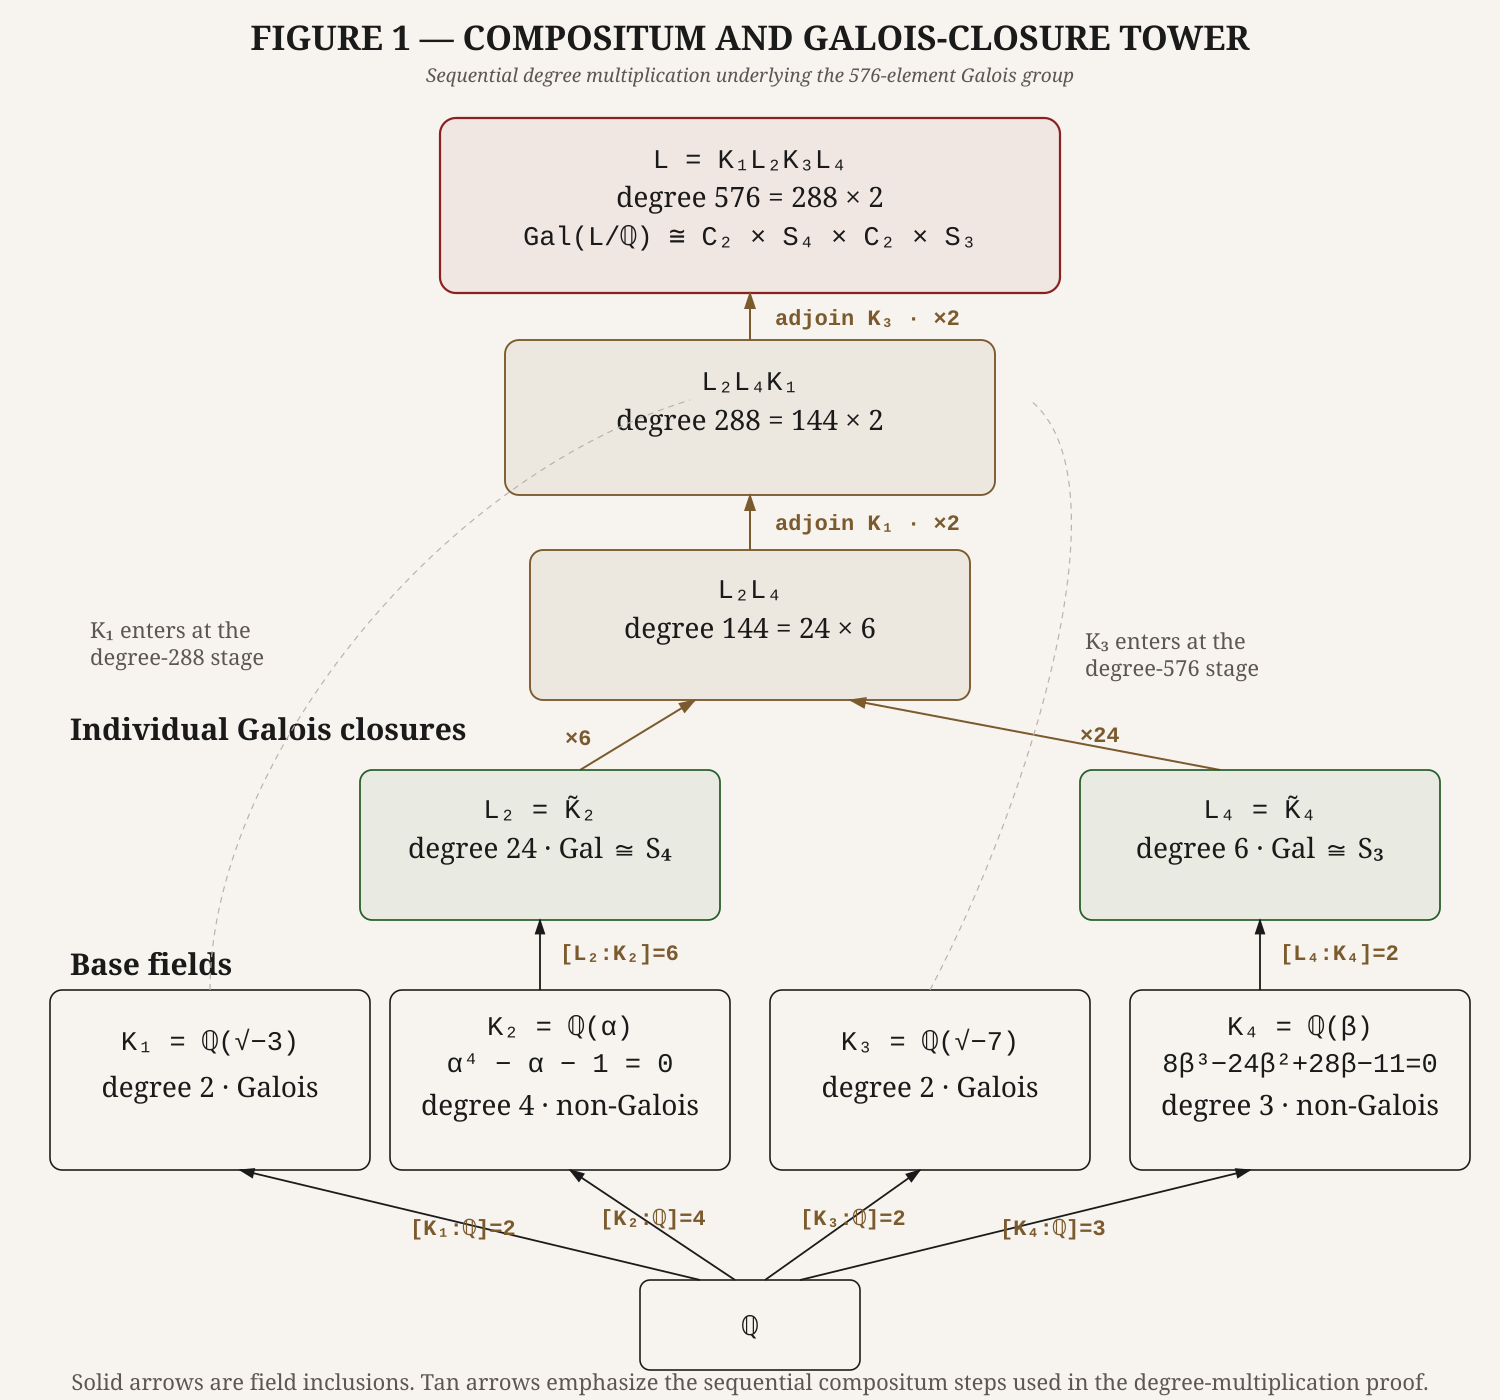
\includegraphics[width=0.96\textwidth]{figure1_compositum_field_tower}
\caption{The Galois-closure tower. The four base fields $K_1,K_2,K_3,K_4$
are extended to their Galois closures $L_2$ (degree~24) and $L_4$ (degree~6),
and the sequential degree chain $[L_2 L_4:\Q]=144$, $[L_2 L_4 K_1:\Q]=288$,
$[L:\Q]=576$ establishes joint linear disjointness.}
\label{fig:tower}
\end{figure}


\section{Proof of Theorem~\ref{thm:main}}\label{sec:proof}

\subsection{Individual Galois closures}
Both Galois groups can be verified directly, without appeal to computer
algebra.

\emph{$\Gal(L_2/\Q)\cong S_4$.} Modulo $2$, $x^4-x-1$ is irreducible over
$\mathbb{F}_2$, so Frobenius at $2$ acts on the four roots as a $4$-cycle.
Modulo $7$, $x^4-x-1$ factors as a linear times an irreducible cubic, so
Frobenius at $7$ acts as a $3$-cycle. A transitive subgroup of $S_4$
containing a $4$-cycle and a $3$-cycle is all of $S_4$, so
$\Gal(L_2/\Q)\cong S_4$ and $[L_2:\Q]=24$.

\emph{$\Gal(L_4/\Q)\cong S_3$.} Set $t=2\beta-2$; then $t^3+2t+1=0$,
which is irreducible modulo $3$ and has polynomial discriminant $-59$, a
nonsquare. An irreducible cubic with nonsquare discriminant has Galois
group $S_3$ rather than $A_3\cong C_3$, so $\Gal(L_4/\Q)\cong S_3$ and
$[L_4:\Q]=6$.

Both facts are also confirmed independently in SageMath; see~\cite{HFGcode}.

\subsection{Degree-multiplication proof}\label{sec:degree}

\begin{proof}[Proof of Theorem~\ref{thm:main} via degree multiplication]
Since $L_2$ and $L_4$ are Galois over $\Q$ and
$[L_2 L_4:\Q]=144=24\cdot 6=[L_2:\Q][L_4:\Q]$, the fields $L_2$ and
$L_4$ are linearly disjoint. Since
$[L_2 L_4 K_1:\Q]=288=144\cdot 2=[L_2 L_4:\Q][K_1:\Q]$,
$K_1$ is linearly disjoint from $L_2 L_4$. Since
$[L_2 L_4 K_1 K_3:\Q]=576=288\cdot 2=[L_2 L_4 K_1:\Q][K_3:\Q]$,
$K_3$ is linearly disjoint from $L_2 L_4 K_1$. The four Galois
extensions are jointly linearly disjoint, so $L/\Q$ is Galois and
Lemma~\ref{lem:product} gives
$\Gal(L/\Q)\cong C_2\times S_4\times C_2\times S_3$ of order
$2\cdot 24\cdot 2\cdot 6=576$.
\end{proof}

The degree equalities were computed in SageMath:
\begin{verbatim}
sage: x = polygen(QQ)
sage: K2 = NumberField(x^4 - x - 1, 'a2')
sage: K4 = NumberField(8*x^3 - 24*x^2 + 28*x - 11, 'a4')
sage: L2 = K2.galois_closure('b'); L2.degree()
24
sage: L4 = K4.galois_closure('d'); L4.degree()
6
sage: L2.composite_fields(L4)[0].degree()
144
\end{verbatim}
The degrees 288 and 576 follow analogously; a self-contained script
is provided in~\cite{HFGcode}.

\subsection{Ramification proof}\label{sec:ramification}


\begin{figure}[ht]
\centering
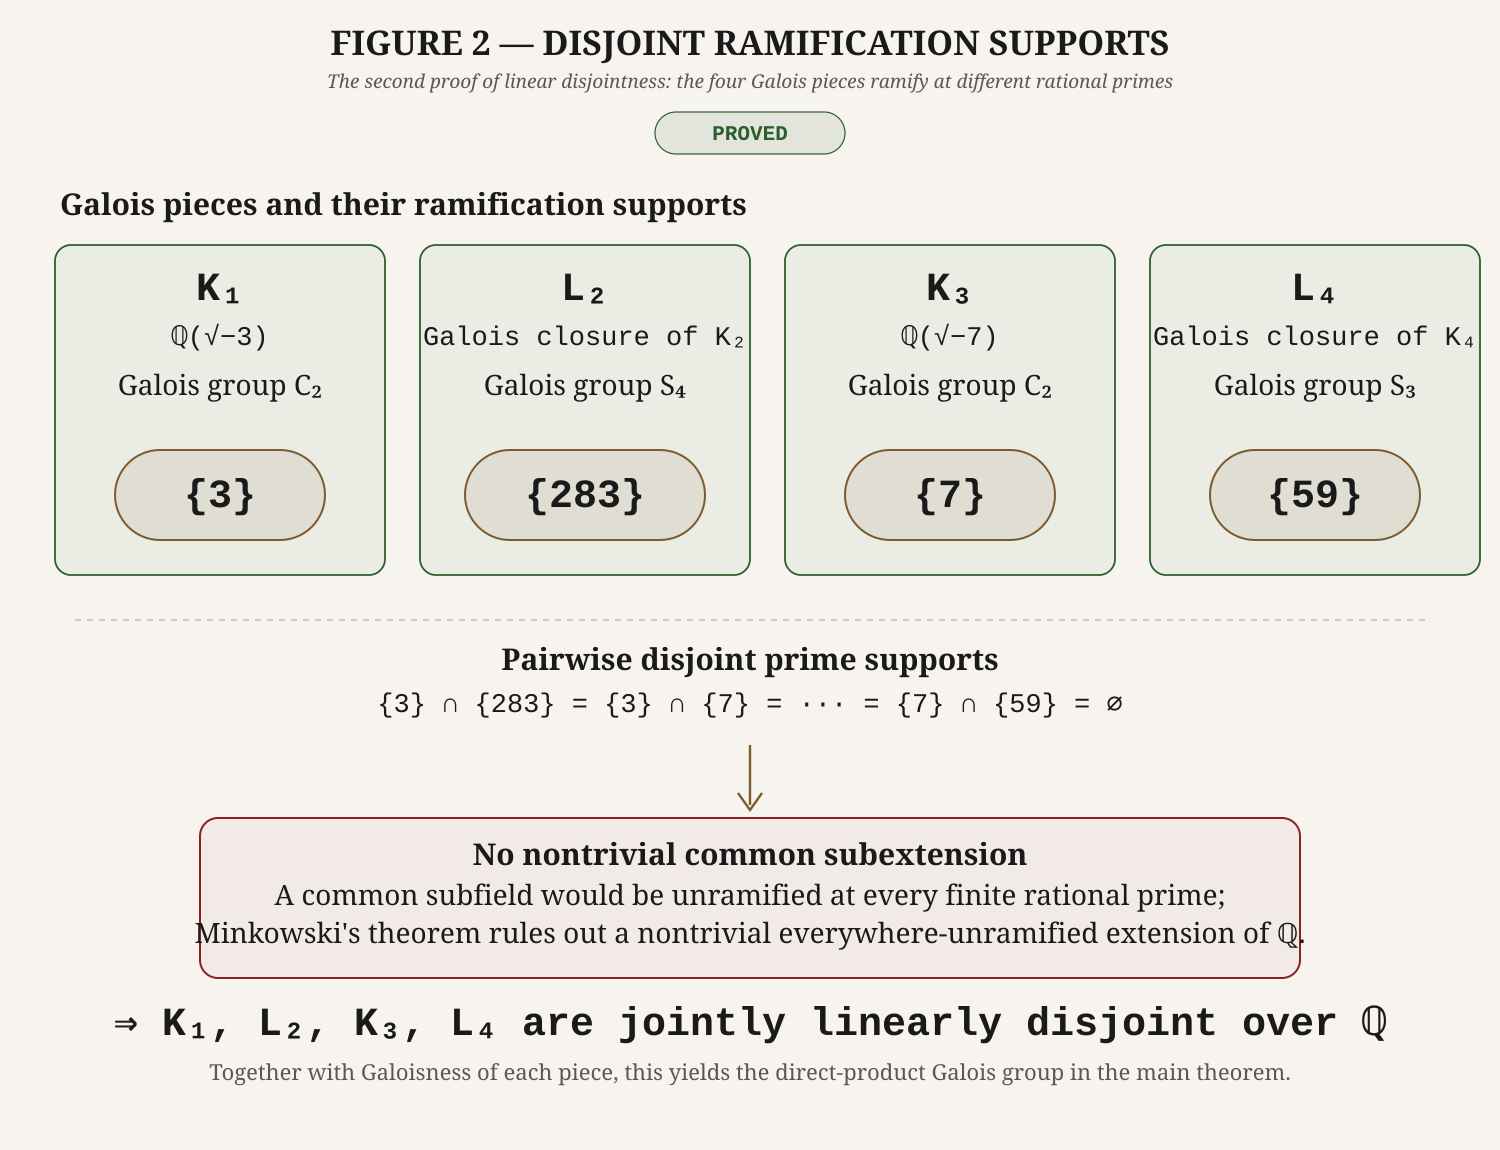
\includegraphics[width=0.96\textwidth]{figure2_ramification_disjointness}
\caption{The four Galois pieces and their disjoint prime ramification
supports. Since no prime is shared between any two pieces, any intersection
would be an unramified extension of $\Q$, which must be trivial by
Minkowski's theorem.}
\label{fig:ramification}
\end{figure}
\begin{proof}[Proof of Theorem~\ref{thm:main} via ramification]
The discriminants of the four Galois pieces are
\[
\disc(K_1)=-3,\qquad \disc(L_2)=283^{12},\qquad \disc(K_3)=-7,\qquad
\disc(L_4)=-59^3
\]
(all verified by SageMath), so their ramification sets $\{3\}$,
$\{283\}$, $\{7\}$, $\{59\}$ are pairwise disjoint. Pairwise disjoint
ramification alone does not imply joint linear disjointness in general,
so we argue by induction. Order the pieces $E_1=K_1$, $E_2=L_2$,
$E_3=K_3$, $E_4=L_4$ and set $F_r=E_1\cdots E_r$. The base case $F_1=E_1$
is trivial. Suppose $F_r/\Q$ is Galois with
$\Gal(F_r/\Q)\cong\prod_{i\le r}\Gal(E_i/\Q)$; in particular every finite
prime ramified in $F_r$ divides $\disc(E_i)$ for some $i\le r$. Since the
ramification set of $E_{r+1}$ is disjoint from all of these, the
intersection $F_r\cap E_{r+1}$ is unramified at every finite prime, so by
Minkowski's theorem~\cite[Theorem~2.17]{Neukirch}, $F_r\cap E_{r+1}=\Q$.
As $F_r$ and $E_{r+1}$ are both Galois over $\Q$, this trivial
intersection gives $[F_{r+1}:\Q]=[F_r:\Q][E_{r+1}:\Q]$ and
$\Gal(F_{r+1}/\Q)\cong\Gal(F_r/\Q)\times\Gal(E_{r+1}/\Q)$, completing the
inductive step. Taking $r=3$ shows the four pieces are jointly linearly
disjoint, and Theorem~\ref{thm:main} follows as before.
\end{proof}

\section{Further Arithmetic Consequences}\label{sec:consequences}

Let $K=K_1K_2K_3K_4$ denote the compositum of the four stem fields
themselves, as opposed to $L$, the compositum of their Galois closures.

\begin{proposition}\label{prop:stemdegree}
$[K:\Q]=48$.
\end{proposition}
\begin{proof}
Since the Galois closures $K_1,L_2,K_3,L_4$ are jointly linearly disjoint
(Theorem~\ref{thm:main}), so are the stem fields $K_1,K_2,K_3,K_4$,
giving $[K:\Q]=2\cdot4\cdot2\cdot3=48$. Confirmed directly in SageMath via
\texttt{composite\_fields}.
\end{proof}

\begin{corollary}[Relative Galois group]\label{cor:relative}
$[L:K]=12$ and $\Gal(L/K)\cong S_3\times C_2$.
\end{corollary}
\begin{proof}
Since $K_1,K_3$ are already Galois of degree $2=|\Gal(K_i/\Q)|$, the
subgroup of $\Gal(K_i/\Q)$ fixing $K_i$ pointwise is trivial. Inside
$\Gal(L_2/\Q)\cong S_4$, the subgroup fixing $K_2$ pointwise is a point
stabilizer for the natural action on the four roots of $x^4-x-1$, hence
isomorphic to $S_3$; inside $\Gal(L_4/\Q)\cong S_3$, the subgroup fixing
$K_4$ pointwise is a point stabilizer on the three roots of $f_4$, hence
isomorphic to $C_2$ (both verified directly in SageMath). Since
$\Gal(L/\Q)$ is the direct product $C_2\times S_4\times C_2\times S_3$
and $K$ embeds as the corresponding product of stem fields, $\Gal(L/K)$
is the direct product of these four stabilizers,
$\{1\}\times S_3\times\{1\}\times C_2\cong S_3\times C_2$, of order
$12=576/48$.
\end{proof}

\begin{corollary}[Uniform ramification exponent]\label{cor:disc}
\[
v_3(\disc L)=v_7(\disc L)=v_{59}(\disc L)=v_{283}(\disc L)=288,
\]
and consequently
\[
\disc(L)=(3\cdot7\cdot59\cdot283)^{288}=350637^{288}.
\]
\end{corollary}
\begin{proof}
At each ramified prime $p$, exactly one of the four Galois pieces
$G_i\in\{K_1,L_2,K_3,L_4\}$ ramifies, with discriminant exponent
$e_i=v_p(\disc G_i)$ and degree $d_i=[G_i:\Q]$. Since the other three
pieces are unramified at $p$ and linearly disjoint from $G_i$, the
extension $L/G_i$ is unramified at $p$, so the tower formula gives
$v_p(\disc L)=[L:G_i]\,e_i=(576/d_i)\,e_i$. For $p=3$: $d_1=2$, $e_1=1$,
giving $288$. For $p=283$: $d_2=24$, $e_2=12$, giving $288$. For $p=7$:
$d_3=2$, $e_3=1$, giving $288$. For $p=59$: $d_4=6$, $e_4=3$, giving
$288$.
\end{proof}

\begin{corollary}[Maximal abelian subextension]\label{cor:abelian}
The abelianization of $\Gal(L/\Q)$ is $C_2^4$, realized by
\[
A=\Q(\sqrt{-3},\sqrt{-283},\sqrt{-7},\sqrt{-59}),\qquad
[A:\Q]=16,\qquad \Gal(A/\Q)\cong C_2^4,
\]
the maximal abelian subextension of $L/\Q$, containing $15$ quadratic
subfields.
\end{corollary}
\begin{proof}
$S_4^{\mathrm{ab}}\cong C_2$ and $S_3^{\mathrm{ab}}\cong C_2$ (in each
case the commutator subgroup is the alternating group, and the quotient
is the sign map), so
$\Gal(L/\Q)^{\mathrm{ab}}\cong C_2\times C_2\times C_2\times C_2$. The
corresponding fixed field is generated by $\sqrt{-3}$, the unique
quadratic subfield $\Q(\sqrt{-283})$ of $L_2$, $\sqrt{-7}$, and the
unique quadratic subfield $\Q(\sqrt{-59})$ of $L_4$. Directly verified in
SageMath: the compositum of these four quadratic fields has degree $16$
with Galois group $C_2\times C_2\times C_2\times C_2$.
\end{proof}

\section{Weyl Group Corollary}\label{sec:weyl}

The standard isomorphisms
\[
W(\mathrm{SU}(2))\cong C_2,\qquad W(\mathrm{SU}(3))\cong S_3,\qquad
W(\mathrm{SU}(4))\cong S_4
\]
combined with Theorem~\ref{thm:main} give Corollary~\ref{cor:weyl} immediately.

\begin{remark}
The identification of the four Galois factors with physical gauge
sectors---as in the Pati-Salam model
$\mathrm{SU}(4)\times\mathrm{SU}(2)_L\times\mathrm{SU}(2)_R$ together
with $\mathrm{SU}(3)_C$---belongs to the HFG program's physical
interpretation and is not part of the theorem.
\end{remark}

\section{Discussion}\label{sec:discussion}

\subsection{Relationship to the HFG program}
The four fields arise in the Hyperbolic Flavor Geometry
program~\cite{HFG}, which investigates whether Standard Model flavor
parameters are arithmetic invariants of finite-volume cusped hyperbolic
3-manifolds.
The association of $K_1$ with $m003$, $K_2$ with $m019$, $K_4$ with
$m006$, and $K_3=\Q(\sqrt{-7})$ with a candidate right-handed $\mathrm{SU}(2)$
manifold is proposed in that program, building on the arithmetic
independence established in~\cite{DualSurgery}. Theorem~\ref{thm:main} and
Corollary~\ref{cor:weyl} are results in algebraic number theory,
independent of any physical interpretation.

\subsection{Open questions}
\begin{enumerate}
\item \textit{Canonicity of $m010$.} By Proposition~\ref{prop:manifolds},
  $m010$ has invariant trace field exactly $K_3=\Q(\sqrt{-7})$, on the
  same computational footing as the identifications for $m003$, $m019$,
  and $m006$. What remains open is whether $m010$ is the \emph{canonical}
  geometric representative for this factor---in particular, whether it is
  the unique minimal-volume census manifold with this trace field.
\item \textit{Covering tower structure.} The manifolds $m003$ and $m006$
  have covering towers with Lucas-number behavior in their first homology
  groups~\cite{MR97}. Whether an analogous structure extends to the
  four-field compositum is open.
\item \textit{Geometric mechanism.} The theorem establishes an algebraic
  isomorphism. Whether a 3D-3D correspondence in the sense of
  Dimofte-Gaiotto-Gukov provides a geometric mechanism elevating this
  to a dynamical statement about gauge interactions remains an open
  problem.
\end{enumerate}

\section*{Appendix: Chebotarev Density Check}

As a further empirical check on Theorem~\ref{thm:main}, the direct-product
structure predicts, by the Chebotarev density theorem, that the density
of rational primes splitting completely in $L$ is $1/576$. Testing all
$3241$ unramified primes below $30000$: the four defining polynomials
split completely simultaneously at exactly $5$ primes, against an
expected count of $3241/576\approx5.63$ under the theoretical density---
consistent with, though of course not an independent proof of,
Theorem~\ref{thm:main}.

\section*{Acknowledgments}
The author used Claude (Sonnet 4.6) as a research
assistant for editorial support and computational verification in
preparing this manuscript. All mathematical content, proofs, and scientific
claims are the author's own work, independently verified using SageMath
and SnapPy.

\begin{thebibliography}{99}
\bibitem{MR}
C.~Maclachlan and A.~W.~Reid,
\emph{The Arithmetic of Hyperbolic 3-Manifolds},
Graduate Texts in Mathematics~219, Springer, New York, 2003.
\bibitem{MR97}
C.~Maclachlan and A.~W.~Reid,
Generalised Fibonacci manifolds,
\emph{Transform.\ Groups} \textbf{2} (1997), no.~2, 165--182.
\bibitem{NR}
W.~D.~Neumann and A.~W.~Reid,
Arithmetic of hyperbolic manifolds,
in \emph{Topology '90} (Columbus, OH, 1990),
Ohio State Univ.\ Math.\ Res.\ Inst.\ Publ.~1,
de~Gruyter, Berlin, 1992, pp.~273--310.
\bibitem{Neukirch}
J.~Neukirch,
\emph{Algebraic Number Theory},
Grundlehren der Mathematischen Wissenschaften~322,
Springer, Berlin, 1999.
\bibitem{SnapPy}
M.~Culler, N.~M.~Dunfield, M.~Goerner, and J.~R.~Weeks,
SnapPy, a computer program for studying the geometry and topology
of 3-manifolds, \url{http://snappy.computop.org}.
\bibitem{HFG}
M.~Gentry,
Hyperbolic Flavor Geometry research program,
\url{https://hyperbolicflavorgeometry.org}.
\bibitem{HFGcode}
M.~Gentry,
HFG computational suite,\\
\url{https://github.com/drmlgentry/hyperbolic-flavor-geometry},
commit \texttt{e0bfd33} (2026).
\bibitem{DualSurgery}
M.~Gentry,
The Meyerhoff manifold as a dual Dehn filling of two
arithmetically independent cusped parents,
preprint, SSRN~7277458 (2026),\\
\url{https://doi.org/10.2139/ssrn.7277458}.
\end{thebibliography}
\end{document}
